\documentclass[11pt,a4paper]{article}
\usepackage[T1]{fontenc}
\usepackage[utf8]{inputenc}
\usepackage{lmodern}
\usepackage[margin=1in]{geometry}
\usepackage{microtype}
\usepackage{amsmath,amssymb}
\usepackage{graphicx}
\usepackage{booktabs}
\usepackage{tabularx}
\usepackage{longtable}
\usepackage{array}
\usepackage[font=small,labelfont=bf]{caption}
\captionsetup[table]{position=top,skip=4pt}
\usepackage[authoryear,round]{natbib}
\usepackage{xr-hyper}
\externaldocument{audit}
\usepackage[hidelinks]{hyperref}
\usepackage{xurl}
% archived copies of web sources, written by tools/archive_sources.py
\makeatletter
\newcommand{\archiveurl}[2]{\@namedef{arch@#1}{#2}}
\newcommand{\archived}[1]{\@ifundefined{arch@#1}{}{. Archived at \expandafter\url\expandafter{\csname arch@#1\endcsname}}}
\makeatother
\InputIfFileExists{archive_urls.tex}{}{}
\newcolumntype{L}{>{\raggedright\arraybackslash}X}
\newcolumntype{P}[1]{>{\raggedright\arraybackslash}p{#1}}
\setlength{\parskip}{0.35em}

\renewcommand{\thesection}{S\arabic{section}}
\renewcommand{\thetable}{S\arabic{table}}
\renewcommand{\thefigure}{S\arabic{figure}}

\title{Supplementary material for\\``What the 50 Best Restaurants list can and cannot resolve:\\a sensitivity audit of its voting system''}
\author{Samuele Lo Piano}
\date{}

\begin{document}
\maketitle

\noindent Section~\ref{app:intervals} lists the simulated rank interval of every restaurant of the 2026 list, and Section~\ref{app:ot} reports the optimal-transport sensitivity indices of Section~\ref{sec:gsa} of the paper. Code and data are at \url{https://github.com/Confareneoclassico/50best-voting-audit}.

\section{The 2026 list with simulated rank intervals}\label{app:intervals}

{\small
\begin{longtable}{@{}rllrr@{}}
\caption{Published 2026 position, 5th to 95th percentile of the simulated position under the published rules (pooled over the six worlds of Section~\ref{sec:gsa}), and the probability of a top-50 place.}\label{tab:intervals}\\
\toprule
Rank & Restaurant & City & 90\% interval & P(top 50) \\
\midrule
\endfirsthead
\toprule
Rank & Restaurant & City & 90\% interval & P(top 50) \\
\midrule
\endhead
\bottomrule
\endfoot
1 & Asador Etxebarri & Atxondo & 1--1 & 1.00 \\
2 & Gaggan & Bangkok & 2--3 & 1.00 \\
3 & Alchemist & Copenhagen & 2--4 & 1.00 \\
4 & Quintonil & Mexico City & 3--5 & 1.00 \\
5 & Wing & Hong Kong & 4--9 & 1.00 \\
6 & The Chairman & Hong Kong & 5--10 & 1.00 \\
7 & Kjolle & Lima & 5--12 & 1.00 \\
8 & Kadeau & Copenhagen & 5--12 & 1.00 \\
9 & Diverxo & Madrid & 6--16 & 1.00 \\
10 & Plénitude & Paris & 8--16 & 1.00 \\
11 & Atomix & New York & 7--17 & 1.00 \\
12 & Sorn & Bangkok & 8--22 & 1.00 \\
13 & Mérito & Lima & 9--22 & 1.00 \\
14 & Sühring & Bangkok & 9--24 & 1.00 \\
15 & Odette & Singapore & 11--28 & 1.00 \\
16 & Tuju & São Paulo & 10--30 & 1.00 \\
17 & Mingles & Seoul & 11--30 & 0.99 \\
18 & Nusara & Bangkok & 13--34 & 0.99 \\
19 & Jan & Munich & 14--40 & 0.97 \\
20 & Piazza Duomo & Alba & 14--38 & 0.98 \\
21 & Meet the Bund & Shanghai & 13--45 & 0.97 \\
22 & Boragó & Santiago & 14--52 & 0.93 \\
23 & Vyn & Skillinge & 14--45 & 0.96 \\
24 & Al Gatto Verde & Modena & 14--46 & 0.97 \\
25 & Lasai & Rio de Janeiro & 14--50 & 0.95 \\
26 & Masque & Mumbai & 18--56 & 0.91 \\
27 & Reale & Castel di Sangro & 20--61 & 0.89 \\
28 & Trèsind Studio & Dubai & 17--65 & 0.89 \\
29 & Enigma & Barcelona & 15--68 & 0.89 \\
30 & Steirereck & Vienna & 20--58 & 0.88 \\
31 & Celele & Cartagena & 18--72 & 0.79 \\
32 & Potong & Bangkok & 22--75 & 0.82 \\
33 & Elkano & Getaria & 19--82 & 0.76 \\
34 & Le Coquillage & Saint-Méloir-des-Ondes & 23--78 & 0.70 \\
35 & La Colombe & Cape Town & 20--78 & 0.76 \\
36 & Ru Yuan & Hangzhou & 21--73 & 0.72 \\
37 & Nuema & Quito & 20--80 & 0.79 \\
38 & Atelier Moessmer Norbert Niederkofler & Brunico & 23--98 & 0.71 \\
39 & Schloss Schauenstein & Fürstenau & 24--86 & 0.60 \\
40 & Jordnær & Copenhagen & 24--110 & 0.60 \\
41 & Onjium & Seoul & 22--91 & 0.69 \\
42 & Bozar & Brussels & 28--86 & 0.60 \\
43 & Le Calandre & Rubano & 29--156 & 0.54 \\
44 & Don Julio & Buenos Aires & 26--98 & 0.55 \\
45 & Mayta & Lima & 22--86 & 0.55 \\
46 & El Chato & Bogotá & 30--133 & 0.46 \\
47 & Le Louis XV - Alain Ducasse & Monte Carlo & 29--137 & 0.47 \\
48 & Ikoyi & London & 27--97 & 0.41 \\
49 & Naar & Kasauli & 27--101 & 0.40 \\
50 & Saint Peter & Sydney & 31--149 & 0.48 \\
51 & Uliassi & Senigallia & 34--114 & 0.39 \\
52 & La Cime & Osaka & 30--120 & 0.36 \\
53 & Ling Long & Shanghai & 35--101 & 0.40 \\
54 & Nelita & São Paulo & 34--127 & 0.29 \\
55 & Alcalde & Guadalajara & 32--138 & 0.39 \\
56 & Sazenka & Tokyo & 35--134 & 0.46 \\
57 & Koan & Copenhagen & 36--169 & 0.23 \\
58 & Frantzén & Stockholm & 30--162 & 0.27 \\
59 & Narisawa & Tokyo & 36--177 & 0.25 \\
60 & Hiša Franko & Kobarid & 32--173 & 0.28 \\
61 & Florilège & Tokyo & 42--184 & 0.14 \\
62 & Fu He Hui & Shanghai & 35--177 & 0.26 \\
63 & The Jane & Antwerp & 38--186 & 0.20 \\
64 & Seroja & Singapore & 40--189 & 0.17 \\
65 & Fyn & Cape Town & 42--174 & 0.12 \\
66 & Willem Hiele & Oudenburg & 39--167 & 0.19 \\
67 & Arpège & Paris & 38--254 & 0.22 \\
68 & Evvai & São Paulo & 42--257 & 0.19 \\
69 & Cocina Hermanos Torres & Barcelona & 40--185 & 0.10 \\
70 & Kol & London & 35--156 & 0.23 \\
71 & Salsify at the Roundhouse & Cape Town & 42--266 & 0.12 \\
72 & Eatanic Garden & Seoul & 41--196 & 0.14 \\
73 & Chef Tam's Seasons & Macau & 42--238 & 0.16 \\
74 & Le Du & Bangkok & 38--189 & 0.12 \\
75 & Belcanto & Lisbon & 40--204 & 0.14 \\
76 & Nobelhart \& Schmutzig & Berlin & 37--168 & 0.14 \\
77 & Caprice & Hong Kong & 44--269 & 0.09 \\
78 & Mosu & Seoul & 42--231 & 0.09 \\
79 & Huniik & Mérida & 47--254 & 0.14 \\
80 & Txispa & Atxondo & 52--225 & 0.04 \\
81 & Septime & Paris & 43--216 & 0.15 \\
82 & Coda & Berlin & 51--277 & 0.04 \\
83 & The Ledbury & London & 54--250 & 0.04 \\
84 & Le Doyenné & Saint-Vrain & 48--260 & 0.07 \\
85 & Tim Raue & Berlin & 44--216 & 0.11 \\
86 & Eliane & Brussels & 43--323 & 0.08 \\
87 & Arca & Tulum & 46--271 & 0.08 \\
88 & FZN & Dubai & 54--281 & 0.03 \\
89 & Burnt Ends & Singapore & 52--252 & 0.03 \\
90 & Baan Tepa & Bangkok & 56--360 & 0.01 \\
91 & Den & Tokyo & 52--247 & 0.04 \\
92 & Lamdre & Beijing & 42--347 & 0.08 \\
93 & SingleThread & Healdsburg & 48--319 & 0.08 \\
94 & Neolokal & Istanbul & 52--324 & 0.05 \\
95 & Mil & Cusco & 64--312 & 0.02 \\
96 & Rosetta & Mexico City & 52--232 & 0.03 \\
97 & Khufu's & Giza & 58--337 & 0.03 \\
98 & Labyrinth & Singapore & 50--333 & 0.05 \\
99 & Fauna & Valle de Guadalupe & 48--299 & 0.07 \\
100 & Aponiente & El Puerto de Santa María & 61--306 & 0.03 \\

\end{longtable}
}

\section{Optimal-transport sensitivity indices}\label{app:ot}

The optimal-transport index of \citet{borgonovo2025ot} compares the distribution of an output $Y$ with its distribution at each level of a factor,
\[
\iota_i = \frac{E\bigl[W_2^2(P_Y, P_{Y \mid x_i})\bigr]}{2\,\mathrm{Var}\,Y},
\]
where $W_2$ is the 2-Wasserstein distance and the expectation runs over the levels of $x_i$, which are equally likely in the factorial design. For a one-dimensional output, $W_2^2$ is the integral over $(0,1)$ of the squared difference of the two quantile functions. We compute it exactly for the empirical distributions of the 6,912 simulated editions and of the 2,304 or 3,456 editions at each level. Writing $m$ and $\sigma$ for the mean and standard deviation of $P_Y$, $m_i$ and $\sigma_i$ for those of $P_{Y \mid x_i}$, and $\rho_i$ for the correlation of the two quantile functions over $(0,1)$, the distance splits into three non-negative parts,
\[
W_2^2(P_Y, P_{Y \mid x_i}) = (m - m_i)^2 + (\sigma - \sigma_i)^2 + 2\,\sigma \sigma_i (1 - \rho_i),
\]
a shift in location, a change in spread and a change in shape. Averaged over the levels and divided by $2\,\mathrm{Var}\,Y$, the location part equals $S_i/2$, so $\iota_i \geq S_i/2$, with equality when a factor only shifts the output. An upper bound follows from coupling $Y$ with the output $Y'$ obtained by drawing $x_i$ again while every other input, the panel included, stays fixed. Then $E[W_2^2] \leq E[(Y - Y')^2] = 2\,S_{Ti}\,\mathrm{Var}\,Y$, so $\iota_i \leq S_{Ti}$ for the total index of the model in which the panel draw is an input. The total indices of Figure~\ref{fig:indices}, computed from cell means, leave out the interactions of a factor with the panel draw and can be smaller. A dummy factor that assigns the simulated editions at random to three levels gives the level of $\iota_i$ that sampling alone produces. Intervals are 95\% jackknife intervals, as in Section~\ref{sec:gsa}.

Table~\ref{tab:ot} and Figure~\ref{fig:ot} report the indices and their parts. Where a factor matters for the rank correlation of the top 100 or the displacement of positions 51 to 100, the location part dominates and the index lies between the two bounds. The vote curve also changes the spread of these two features, which vary more across rules and panels when the top of the list collects fewer votes, and the allocation of voters changes the spread of the number of regions in the top 50.

For the four counts, the shape part is present even where a factor has almost no effect, and for the top ten it makes up most of every index. This is a property of counts that take few values. On the integers, moving probability $p$ from one value to the next costs $p$ in squared distance, while the mean moves by $p$, which enters the location part as $p^2$. A small change in the mean therefore appears mostly as a change in shape. The dummy factor shows the same pattern, with a null level of up to 0.007 on the counts against 0.001 or less on the two continuous features. In the last column of Table~\ref{tab:ot}, each count is smoothed by spreading it uniformly over the unit interval around it before the index is computed. The shape parts then fall to 0.004 or less and the null level to 0.001 or less, and every index of a factor above the null level lies between $S_i/2$ and $S_{Ti}$ of the smoothed count within its interval. The choice of index changes the size of the effects on the counts, then, but not which factors matter.

\begin{figure}[t]
\centering
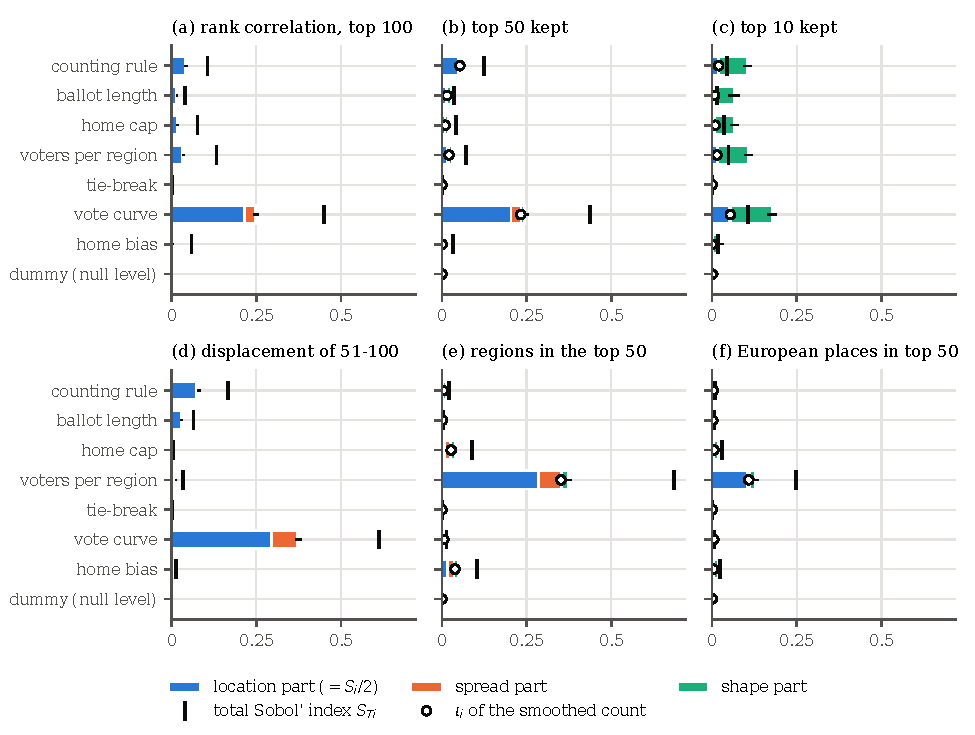
\includegraphics[width=\textwidth]{figures/fig_ot.pdf}
\caption{Optimal-transport indices $\iota_i$ of the six features of the simulated list, split into location, spread and shape parts, with 95\% jackknife intervals. The location part equals $S_i/2$. Ticks: total Sobol' index $S_{Ti}$ of Figure~\ref{fig:indices}. Circles: $\iota_i$ of the counts smoothed by spreading each value uniformly over the unit interval around it. Dummy: runs assigned at random to three levels.}
\label{fig:ot}
\end{figure}

\newpage
{\small
\setlength{\tabcolsep}{4.5pt}
\begin{longtable}{@{}lrcrrrrrr@{}}
\caption{Optimal-transport indices $\iota_i$ with 95\% jackknife intervals, their location, spread and shape parts, the Sobol' indices of Figure~\ref{fig:indices}, and, for the four counts, $\iota_i$ of the count smoothed by spreading it uniformly over the unit interval around it (last column). The bounds for the smoothed index are the Sobol' indices of the smoothed counts, which differ from the $S_i$ and $S_{Ti}$ shown by at most 0.011.}\label{tab:ot}\\
\toprule
Factor & $\iota_i$ & 95\% interval & Location & Spread & Shape & $S_i$ & $S_{Ti}$ & $\iota_i$ smoothed \\
\midrule
\endfirsthead
\toprule
Factor & $\iota_i$ & 95\% interval & Location & Spread & Shape & $S_i$ & $S_{Ti}$ & $\iota_i$ smoothed \\
\midrule
\endhead
\bottomrule
\endfoot
% the primitive input lets the first generated row start with \multicolumn
\csname @@input\endcsname table_ot.tex 
\end{longtable}
}


\bibliographystyle{plainnat}
\bibliography{refs}

\end{document}
